\section{Introducción a OAI-PMH}

\acrfull{oaipmh} (actualmente disponible en su versión 2.0) es un protocolo para la transmisión de metadatos en Internet que surgió del esfuerzo de mejorar y abrir el acceso a archivos de publicaciones electrónicas (e-prints) y en general a un gran rango de materiales digitales que ha despertado el interés de la comunidad de bibliotecarios.\cite{JM_OAI}

El protocolo \acrshort{oaipmh} se basa en una arquitectura cliente-servidor en la que el cliente realiza las consultas por medio de transacciones \acrshort{http} GET o POST constituidas por un conjunto de opciones del tipo clave=valor y se devuelve un documentos \acrshort{xml} bajo al menos el estandar \acrfull{dc} según dicta la especificación de la implementación mínima del protocolo \acrshort{oaipmh} para los proveedores de información.\cite{OAIPMH_implementers}

\begin{figure}[!htp]
	\centering
	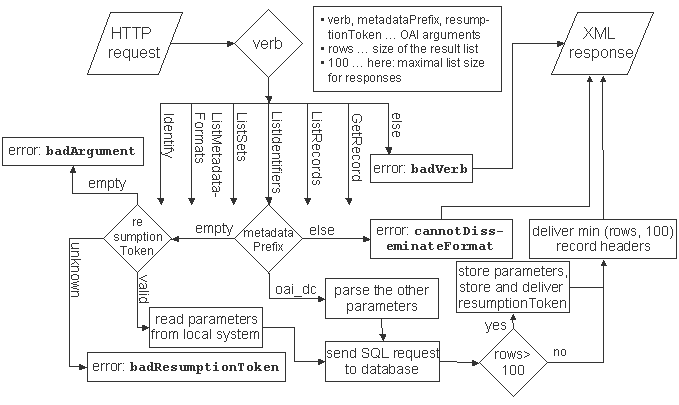
\includegraphics[scale=.5]{fig/oai_flow}
	\caption{Diagrama de flujo del servidor \acrshort{oaipmh}}\label{fig:oaiflow}
\end{figure}

Como se ve en la figura \ref{fig:oaiflow} el cliente puede realizar seis peticiones al servidor en función del valor especificado en el `verb' de la consulta, las peticiones pueden ser:

\begin{itemize}
	\item \textbf{Idenfity:}
	\item \textbf{GetRecord:}
	\item \textbf{ListMetadataFormats:}
	\item \textbf{ListSets:}
	\item \textbf{ListIdentifiers:}
	\item \textbf{ListRecords:}
	\item \textbf{GetRecord:}
\end{itemize}